\documentclass[12pt,preprint]{aastex}
\usepackage{url}
\usepackage{natbib}
\usepackage{graphicx}
\usepackage{subfig}
%\usepackage{fixltx2e}



%%%%%%%%%%%%%%%%%%%%%%%%%%%%%%%%%%%%%%%%%%%%%%%%%%%%
%%% author-defined commands
\newcommand\x         {\hbox{$\times$}}
\def\mic              {\hbox{$\mu{\rm m}$}}
\def\about            {\hbox{$\sim$}}
\def\Mo               {\hbox{$M_{\odot}$}}
\def\Lo               {\hbox{$L_{\odot}$}}

%\captionsetup[figure]{labelformat=simple}
%%%%%%%%%%%%%%%%%%%%%%%%%%%%%%%%%%%%%%%%%%%%%%%%%%%%

% Abstract




\begin{document}

\title{Moving Object Pipeline System Design}

\author{Jonathan Myers, Lynne Jones, Tim Axelrod}

\begin{abstract}

The Moving Object Pipeline System (MOPS) has two responsibilities
within LSST Data Management.  First, it is responsible for generating
and managing the \textbf{Moving Object} data products.  The Moving
Objects are identified solar system objects (SSOs) with associated
Keplerian orbits, errors, and detected sources associated with those
solar system objects.  The second responsibility of the MOPS is to
predict future locations of moving objects in incoming images so that
their sources may be associated with known objects; this will reduce
the number of transient detections and prevent Alert Generation on
detections of known Solar System objects.  Design for the MOPS
component is based closely on the design of the PanSTARRS MOPS.

\end{abstract}

\tableofcontents

%\section{Science Requirements}

\section{System Design and Responsibilities}

The Moving Object Pipeline System has two main responsibilities: the
generation and maintenance of the Moving Object database, and the
prediction of known object locations which are sent to the Association
Pipeline to prevent unneccessary alerts.  The MOPS has been broken
into two components, colloquially known as ``DayMOPS'' and ``NightMOPS.''
Both are based on designs and algorithms in use in the PanSTARRS MOPS
system.
 

\begin{figure}[!ht]
\centering
  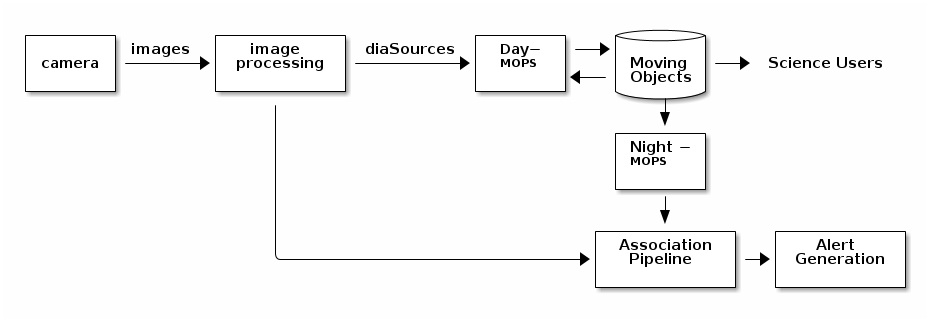
\includegraphics[width=13cm]{illustrations/mopsWithinLsst.png}
\caption{ Data flow from the camera through DayMOPS to the Science
  Users and Alert Generation.  DayMOPS will build and maintain the
  Moving Objects table, NightMOPS will use the Moving Objects table to
  communicate with the Assocation Pipeline.  }
\label{mopsWithinLsst}
\end{figure}


``DayMOPS,'' so called because it processes data acquired from the
previous night in a large batch operation, is responsible for
discovering new Moving Objects in newly-acquired data, searching old
data for detections of new objects, and updating the Moving Objects
table to reflect newly-acquired data. It is also responsible for
periodically cleaning and refining the contents of the Moving Objects
table.  ``NightMOPS'' is responsible for projecting the locations of known
Moving Objects in upcoming images as they are announced during
night-time operations.  

The relationship between DayMOPS, NightMOPS and the neighboring
components of the LSST Data Management system is illustrated in
figure \ref{mopsWithinLsst}.

\subsection{DayMOPS: Discovering and Managing Moving Objects}

% Illustration of DayMOPS

% sky-plane vs. orbit-space illustration

The DayMOPS is responsible for discovering moving objects in source
catalogs.  The task of discovering and tracking asteroids has been
performed by humans since hundreds of years ago, but automated systems
for asteroid discovery and tracking remain relatively uncommon.  Other
surveys have often mixed human and computerized approaches -
\textbf{can we get some more history here?}.


For the LSST DayMOPS, we have chosen to follow the model of the
PanSTARRS Moving Object Pipeline System \citep{psMOPSDesign}.  The
approach used here is to first find sets of detections with sky-plane
paths consistent with asteroid behaviour; these sets of detections and
their fitted paths are called \textbf{tracks}.  A set of algorithms
for the discovery of sky-plane tracks in dense data are presented in
\citet{Kubica:2005:MTA:1081870.1081889}; these algorithms are used in
the PanSTARRS MOPS and the basis of the linking methods for the
current LSST DayMOPS.  

The tracking methods used are based on a tiered approach; first two or
more detections from a single night are linked into
\textbf{tracklets}, which represent a hypothetical object and a linear
approximation of its sky-plane motion.  These tracklets are later
joined into larger tracks.  To suit the needs of orbit fitting, we are
generally only interested in tracks containing tracklets from at least
three nights, and because of the increasing complexity of sky-plane
motion over time, we are generally interested in tracks which span no
more than 15-30 days of observation time.

The PanSTARRS MOPS uses a fairly loose and generous approximation of
asteroid motion.  This allows for many mislinkages or \textbf{false
  tracks}, combining detections which are not attributable to the same
source, but virtually all objects for which a true (correctly-linked)
track could be generated will get some correct track.  With LSST's
expected density of detections, we found that this glut of false
tracks was generally too painful.  As a result, our methods diverge
from those of PanSTARRS as we introduce some more strict filters on
tracks, reducing the number of mislinkages at the expense of
potentially missing some true tracks.  The algorithms, their
implementations, the additional filters, and their behaviors are
presented thoroughly in Chapter \ref{linking}.

Once tracks are discovered, they are sent to the Orbit Determination
phase. The Orbit Determination phase takes these sets of sky-plane
detections and attempts to find a Keplerian orbit which could generate
the detections.  This orbit is further refined, and error bounds are
established, using differential correction.  Orbit Determination will
reject many tracks as false, but should successfully find precise
orbits for virtually all correctly linked tracks.  Several methods for
performing this task are known, and several have open-source implementations
available to LSST \citep{Milani04orbitdetermination},
\citep{Milani2006}, \citep{OpenOrb2009}, \citep{granvik_thesis}.  The
orbits discovered by Orbit Determination, and the detections present
in the track associated with each orbit, are used to generate new
Moving Objects.

\begin{figure}[h]
\begin{center}
  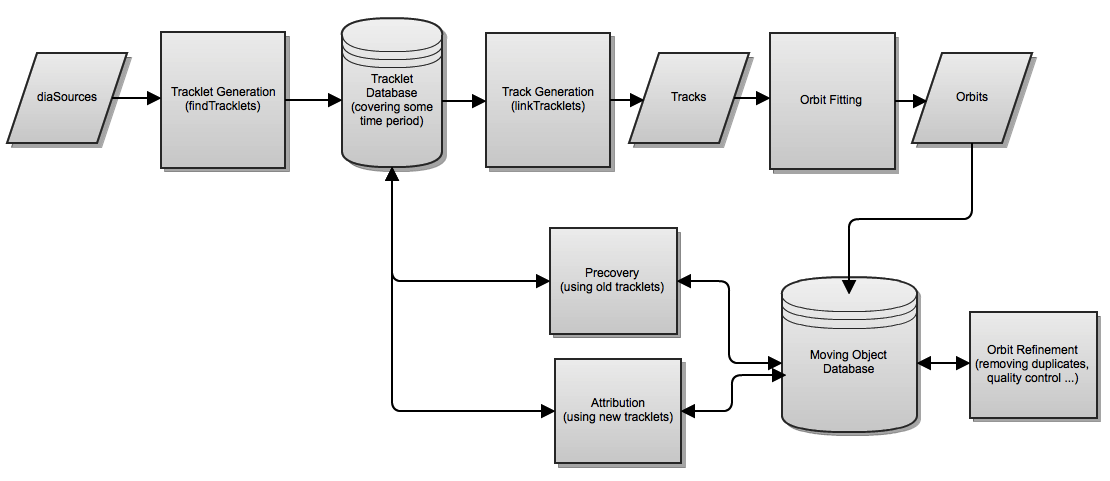
\includegraphics[width=11cm]{illustrations/mopsDiagram.png}
\end{center}
\caption{ Data flows into the DayMOPS pipeline and results in
  modifications of the Moving Objects table in a variety of ways,
  including attribution to known objects, a multi-stage pipeline for
  the discovery of new objects, and periodic refinements of the Moving
  Object table, such as possible merges of redundant objects or
  removal of false orbits. }
\label{mopsDiagram}
\end{figure}



As in the PanSTARRS MOPS design \citep{psMOPSDesign} the LSST's
DayMOPS is expected to perform several additional tasks to manage and
improve the Moving Objects table over time.  Attribution is the
process of identifying known objects in incoming data and adding those
detections to the correct Moving Object (this task is delegated to
NightMOPS). Similarly, Precovery is the recovery of known,
unattributed detections associated with a newly-discovered Moving
Object.  Another refinement is the merging of potentially redundant
Moving Objects.  The complete set of DayMOPS tasks and their data
flows are illustrated in figure \ref{mopsDiagram}.





\subsubsection{Orbit Fitting}
\label{orbitFitting}

Orbits are 6 parameter Keplerian orbits fit to the set of observations
linked during the track building phase. The Keplerian orbit sets
tighter and more complicated constraints on the linkages than the
previous quadratic approximation to this motion, and thus provides a
final filter on linkages which can correspond to true, physical
objects. Using a well-determined orbit, we can predict the location of
an object at arbitrary times.

Orbit fitting can be accomplished using either traditional geometric
methods, where an ellipse or parabola consistent with movement in the
gravitational field of the sun is fit to the set of detections, or
with statistical ranging, where a wide range of potential orbits are
evaluated against the set of detections to search for those with
the lowest residuals. Traditional methods are typically much speedier,
and are available to LSST through the OrbFit software from Milani
\citep{Milani2006}. Statistical ranging methods are more accurate in
exploring the full range of orbital uncertainties for each object,
which can be particularly important for objects observed near 60--90
degrees from the Sun where NEO and MBA exhibit similar apparent
motions, and are available in the OpenOrb software from Granvik
\citep{OpenOrb2009}.

In general, orbit fitting is split into two conceptual pieces - an
``initial orbit determination'' stage, where approximate orbits are
calculated, and a ``differential correction'' stage, where
perturbations on the initial orbit are evaluated to find the best fit
and uncertainty. With six observations on three different nights, most
real moving objects will pass both initial orbit determination and
differential correction with an orbit accurate enough to generate
predicted positions with uncertainties of less than a few arcminutes
for the next few months \citep{basicSolarSystem}.





\subsubsection{Sky-Plane Motion Limits Imposed by Sky-Plane Linking Methods}

Practical considerations necessitate that we set upper bounds on
tracklet velocity and track acceleration in order to restrict the
number of potential mislinkages. Existing methods attempt to find all
tracklets or tracks within specified velocity and acceleration limits;
as velocity and acceleration limits are raised, the number of
tracklets and tracks can grow quickly.  As a result, the choice of
velocity and acceleration limits is important, as it significantly
impacts the objects found as well as the cost of running the software.

Generally, all types of solar system objects except for the fastest of
near-earth asteroids tend to have reasonably low sky-plane velocity
and acceleration. It is expected that the fastest-moving objects will
leave visible trails in images; these may be used to isolate
detections which could be attributable to fast-movers and restrict the
potential search space for linking these detections.  See section
\ref{neosTrailing} for more information on future plans for
approaching this problem.  





\subsection{NightMOPS: Predicting Moving Object Locations}

The NightMOPS section of MOPS is responsible for predicting the
locations of known Moving Objects as images are taken, so that they
may be attributed to the known Moving Objects and removed from the set
of unknown transients detections.  This allows attribution for known
Moving Objects, improving the quality of the Moving Object data
products, and also allows the prevention of unnecessary Alerts.

Predicting the locations of objects given an orbit can be accomplished
through ephemeris calculation using existing orbit-space software
suites \citep{Milani2006}, \citep{OpenOrb2009}.  However, ephemeris
calculation can be fairly slow for large data sets.  Because the
observations schedule for LSST will be determined dynamically, it is
necessary to generate ephemeris predictions for a potentially large
Moving Object table in a short period of time.

% some kind of time-domain illustration?

In order to accomplish this, NightMOPS will generate ``coarse
ephemerides'' for known objects, predicting their locations at the
beginning and end of the night.  Then, when given an upcoming image
location, NightMOPS will use interpolation of the coarse ephemerides
to find objects which could feasibly be present in the upcoming
image. Precise ephemerides for just these objects will be
generated. In this way, NightMOPS will avoid the problem of generating
ephemeris for each known Moving Object for every image time.


\subsection{Implementation Status}

All software components of MOPS, with the possible exception of
initial orbit determination, differential correction, and ephemeris
generation, are expected to be completed in open-source C++ compliant
with LSST software guidelines and in LSST appropriate coding style.
These components will run inside the LSST Pipeline Framework.

Currently, the initial tracking phases of DayMOPS are implemented in
LSST-compliant C++.  The selection of an appropriate package for
initial orbit determination, orbital differential correction, and
ephemeris generation is incomplete but several FORTRAN options are
available to us, some open-source \citep{Milani2006}
\citep{OpenOrb2009}.  A Python-based implementation of NightMOPS,
using the LSST Pipeline Framework, is complete but it is currently
using a closed-source ephemeris generation tool.



\section{Linking of Detections}
\label{linking}



\subsection{Building Tracklets}

% possible illustration: show Dec/time for two images, then tracklets in Dec/time

\textbf{Tracklets} are the building blocks of the sky-plane
\textbf{tracks} used by DayMOPS.  Tracklets are linkages between
DiaSource detections occuring within the same night; during this time
period, solar system object motion is linear or near-linear on the
sky. By creating tracklets, DayMOPS can find sky-plane position and
velocity estimates for sets of detections which may belong to solar
system objects.  This filters out many detections of non-solar system
objects, as they are less likely to generate tracklets.  The use of
tracklets also simplifies the downstream work of track generation,
which attempts to find sets of detections with a good
position/velocity/acceleration fit on the sky-plane; since tracklets
have known position and velocity, the track generation phase needs
only to find those tracklets compatible within some acceleration
factor.

In order to ensure that tracklet-generating images are acquired, it is
necessary to ensure that regions of the sky are visited two or more
times within an accepted time period each night.  Currently, we
require that sky fields be revisited within a fairly short time period
($\leq 90$ minutes is the current rule) in order to constrain the
maximum apparent motion of solar system objects and thus also
constrain the number of tracklets.

The discovery of tracklets can be accomplished efficiently using
KD-Tree structures \citep{bentley_kdtrees} and methods from
\citet{kubica_thesis}.  DayMOPS will build a 2-dimensional (RA, Dec)
KD-Tree for each image, using the tree to hold the detections found in
that image.  Because KD-Trees allow quick range searches of
arbitrary-dimensional spatial data, it is possible to efficiently
perform searches over the detections to find pairs of detections
sufficiently close within time and within limits on apparent
velocity. These pairs of detections are linked to generate tracklets.
% TBD: Is this clear?!

% psuedo code?

Further refinements of tracklets are possible with additional
processing. If an object gets more than one tracklet, it is possible
to use methods similar to the Hough transform to identify and merge
these redundant tracklets into larger tracklets, improving the linear
position/velocity fits of the tracklets and reducing the number of
tracklets passed downstream.

\subsection{Building Tracks}

Over the course of roughly one month, solar system objects tend to
follow a roughly quadratic path on the sky-plane
\citep{kubica_thesis}.  The track generation phase of DayMOPS will
attempt to find sets of tracklets (which have position and velocity
estimates) which were observed within one month of each other and are
compatible within some acceleration range.  Tracks which are
suitable for generating a reasonable orbital fit are sent to the Orbit
Determination phase.

The methods used for tracklet-to-tracklet linking are described in
\citet{kubica_thesis} and \citet{Kubica:2005:MTA:1081870.1081889}.
The methods described attempt to efficiently find sets of tracklets
which are \textit{compatible} in the sense that they could be joined
to form a track: that is, tracklets which span multiple nights and
have positions and velocities which are consistent with a fixed
acceleration.  

To perform this work efficiently, these methods use four-dimensional
KD-Trees over \textit{tracklet-space}, or (RA position, Dec position,
RA velocity, Dec velocity). One tree is created per image, and holds
each tracklet which has its first detection in that image.  A
multi-tree walk is performed using a clever algorithm, efficiently
discovering all regions of tracklet-space which could contain sets of
tracklets that are compatible, while avoiding visits to tracklet-space
regions which are not compatible and could not generate a track.  This
is performed recursively until leaf nodes of the KD-Trees are reached.

% illustration from Kubica?

When the algorithm encounters a set of leaf nodes in the KD-Trees, it
attempts to build a track using the detections held in the tracklets
at the leaf nodes.  A quadratic fit, or a higher-order fit if
possible, to the detections will be attempted.  Then a quality-of-fit
assessment is used to determine whether the track is considered
sufficiently well-fitted to pass downstream to the Orbit
Determination.  Investigation into ideal higher-order fits and
quality-of-fit metrics is ongoing, but as of this writing a filter on
minimum chi-squared probability appears to be the best option.




\subsection{Metrics \& Scaling of Sky-Plane Linking Methods}

Current development efforts have focused on the sky-plane tracking
phase of DayMOPS, as all later processing is dependant on its
success. Existing orbit determination packages claim a high rate of
success for accurate Orbit Determination (OD) given a correctly-linked
track, and should correctly reject false tracks in nearly all cases
\citep{Milani2006}. As a result, we expect that the ability of the
system to successfully generate Moving Objects data products for solar
system objects given to DayMOPS will be determined primarily by the
sky-plane tracking component and its ability to send useful tracks to
OD.  We also expect the overall resource usage of the DayMOPS system
will be calculable given the runtime of the sky-plane tracking
component, the number of tracks it passes to OD, and the per-track OD
time of our OD package.  As a result, carefully studying the behavior
and output of the sky-plane linking should provide a reasonable
estimate of the resource usage of all of DayMOPS object discovery.

% NightMOPS RESOURCE USAGE?!

In this section, we will present metrics used to evaluate the
usefulness of the sky-plane tracking approach, the correctness of our
software implementation, and usefulness of filters. We also
investigate the expected resource usage of our software and expected cost
of performing OD on its output.



\subsubsection{Experiments And Results}

\subsubsubsection{Metrics for End-to-end Evaluation of Sky-plane Linking}
MOPS can generate a useful orbit, and thus a Moving Object, for an
object if it is observed sufficiently for OD to be performed (see
\ref{cadenceRequirements} for details) and a track containing those
observations is correctly generated by DayMOPS and passed to its OD
phase.  An object for which such a track is generated by DayMOPS is
considered to be \textbf{found} by the DayMOPS pipeline.  

Despite the best efforts of the telescope's cadence, not all objects
are observed in a manner such that they can generate an OD-worthy
track.  We refer to an object which is observed with a cadence
sufficient for an OD-worthy track as a \textbf{findable} object.  When
running simulations, determining whether or not a given object is
findable is fairly straightforward: by using \textit{a priori}
knowledge of when its simulated detections occurred, we can simply
measure the time intervals between these detections and determine
whether the time interval were sufficient for tracklet generation and
track generation.  Note that the sky-plane velocities/accelerations of
the objects are \textit{not} used in deciding whether an object is
considered findable.


To understand net cost and success of our linking, the number of
objects found and the cost of finding them is likely sufficient.
However, when measuring and optimizing the internal behavior of the
DayMOPS system, it is helpful to study the quality and quantity of the
intermediate data structures used. Thus, we present a few additional
metrics as well.

The total number of tracks or tracklets is of significant concern when
estimating the resource usage of the system.  The number of tracklets
will be a major factor in the predicting the workload of track
generation, and the number of tracks should entirely decide the size
of the workload for OD.  As such, we measure the \textbf{number of
  tracks} and \textbf{number of tracklets}.  

Correctly-linked tracks and tracklets are referred to as \textbf{true
  tracks} and \textbf{true tracklets}. We present the percentage of
tracklets and tracks which are true in our results. Note that it is
expected that multiple correctly-linked tracklets and/or tracks may be
generated for a given found object. As such, we expect the number of
true tracks and tracklets to significantly exceed the number of found
objects.  Nonetheless, we find that checking the true/false ratio of
tracklets and tracks helps to illustrate the quality of linkages used
as input to the track generation software and to OD.

%% \textbf{consider a paragraph on object coverage; we will need to
%%   update my existing code if we use it.}




\subsubsection{Results From Main-Belt and Distant Object Searching On Ecliptic}

The ecliptic plane is the most densely-populated region of the sky,
and main-belt asteroids generate the vast majority of detected objects
there.  We chose to run a simulated one-year survey using simulated
images from a section of the ecliptic.  

The survey was intended to search for main-belt asteroids, on the
expectation that if they could be found and removed the clutter of the
images would be significantly reduced. This should render further
searching (say, for fast-moving near earth objects) less challenging.
Further, because our software looks for objects moving or accelerating
\textit{below} a set threshold, objects moving and accelerating more
slowly than main-belters were also found.

\subsubsubsection{Choosing the Linking Time-Window}

As expected in production, we attempted to generate tracklets between
any pair of images separated by more than 15 minutes and less than
90 minutes.  However, to speed up the track generation phase, we
attempted to link tracklets if they were separated by $\leq$ 15 days;
in production, it is expected that this number will be 30.  These
numbers should be consistently true across all experiments presented
here.


\subsubsubsection{Choosing Velocity and Acceleration Limits}
\label{velAccLimits}
\begin{figure}[ht!]
  \centering
  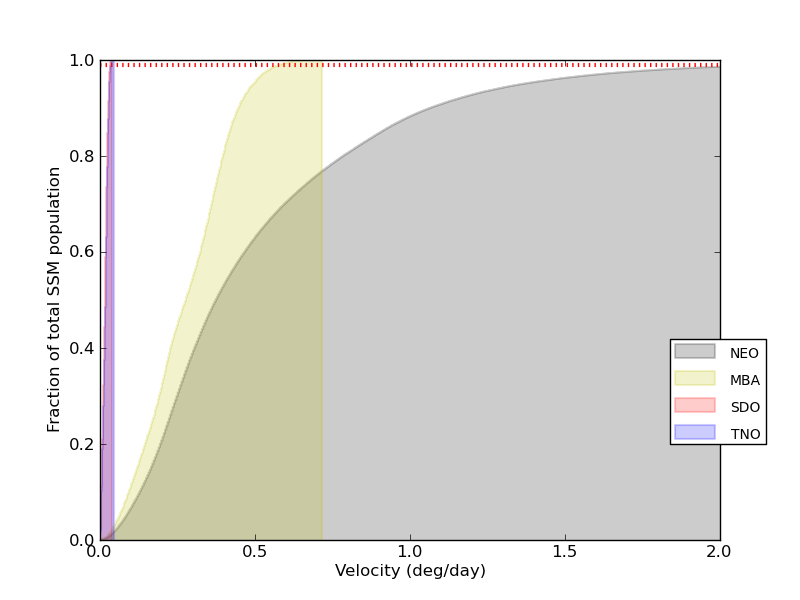
\includegraphics[width=13cm]{illustrations/mopsplots/aug2011/n_velocity.png}
  \caption{A cumulative histogram of solar solar system object
    sky-plane velocities, organized by classification.  Note that only
    the near-earth objects have higher velocities than main-belt
    asteroids.}
  \label{velSurvey}
\end{figure}

\begin{figure}[ht!]
  \centering
  \subfloat[Apparent Accelerations in Right Ascension over 15 Days]{
    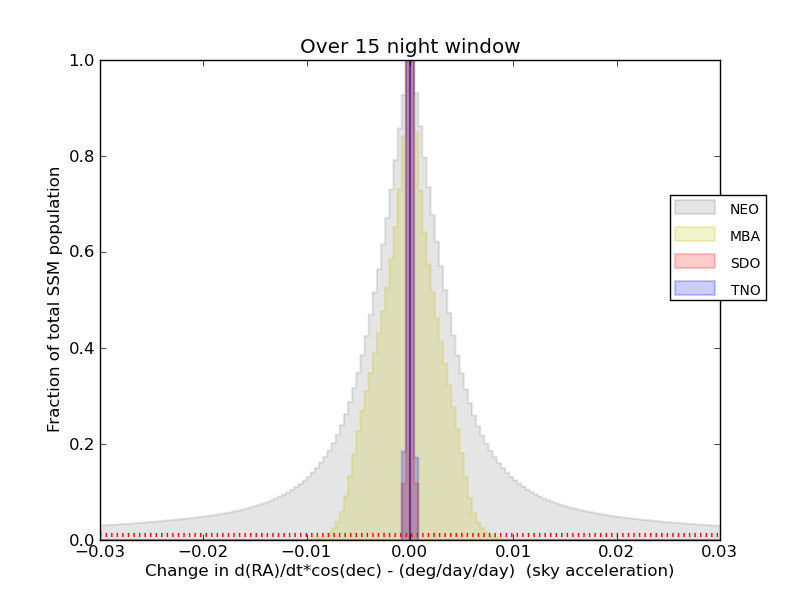
\includegraphics[width=8cm]{illustrations/mopsplots/aug2011/n_accel_ra_15.png}
    }
  \subfloat[Apparent Accelerations in Right Ascension over 30 Days]{
    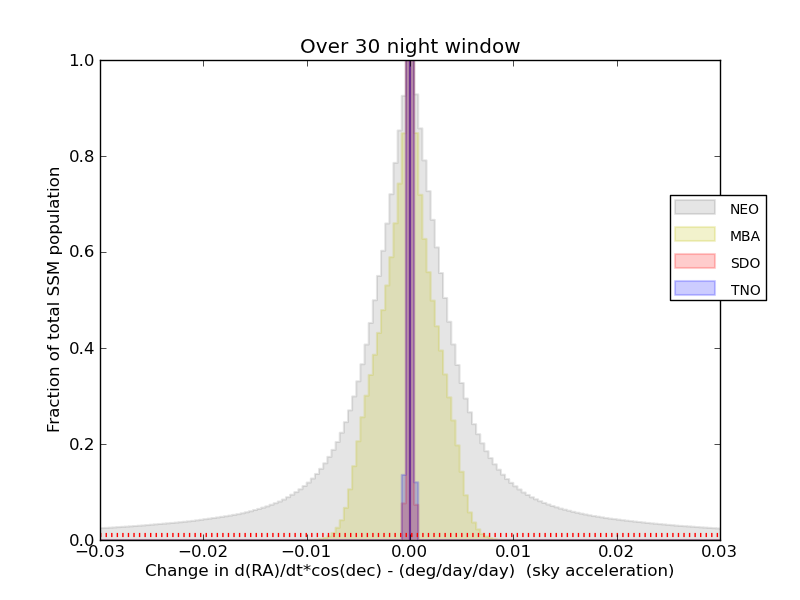
\includegraphics[width=8cm]{illustrations/mopsplots/aug2011/n_accel_ra_30.png}
    }

  \subfloat[Declination Apparent Accelerations in Declination over 15 Days]{
    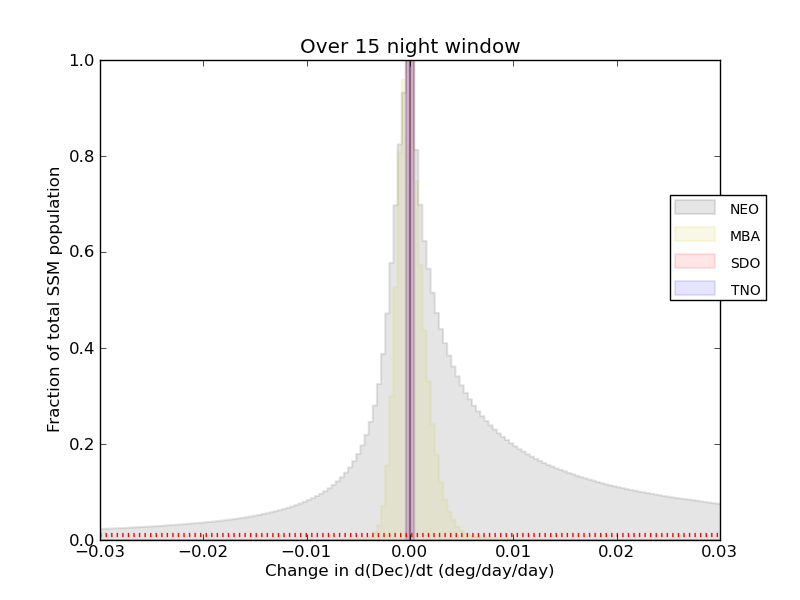
\includegraphics[width=8cm]{illustrations/mopsplots/aug2011/n_accel_dec_15.png}
    }
  \subfloat[Declination Apparent Accelerations in Declination over 30 Days]{
    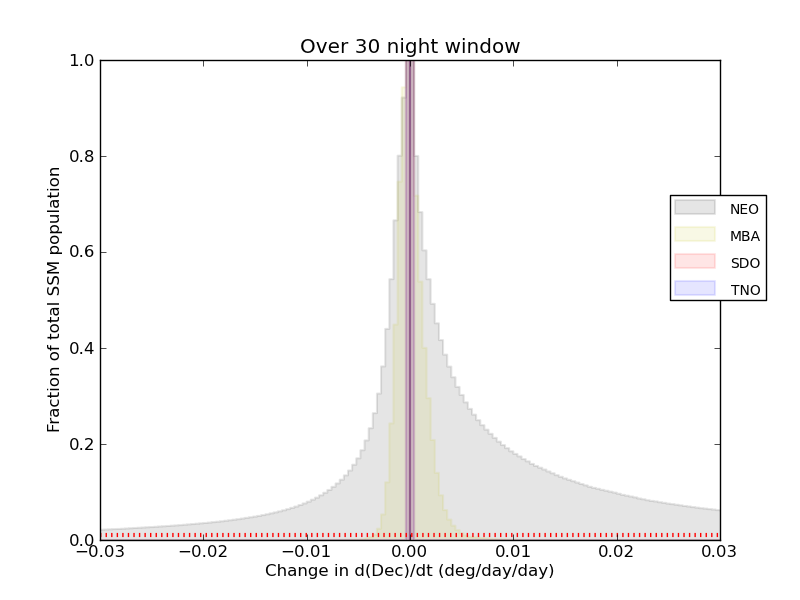
\includegraphics[width=8cm]{illustrations/mopsplots/aug2011/n_accel_dec_30.png}
    }
  \caption{Normalized histograms of sky-plane accelerations of several
    classes solar system objects in the RA and declination, with
    objects grouped by classification.  Histograms are presented for
    changes over 15 days and 30 days. The best-fit accelerations vary
    slightly given the size of the window; this is due to
    non-quadratic factors not included in the simple quadratic model.
    15 day tracking windows are used in the experiments presented in
    this document, but we expect to move to 30 day windows in the
    future.  In both cases, virtually all MBAs, and all other objects
    except NEOs, should have accelerations between -.02 and .02
    deg/day$^2$ in both axes.}
  \label{accSurvey}
\end{figure}


In order to determine reasonable limits on velocity and acceleration
of various classes of solar system objects, a survey of the solar
system model \citep{Grav2011} was conducted, see figures
\ref{velSurvey}, \ref{accSurvey} for histograms
presenting the results of these surveys.

We found that a velocity limit of .5 deg/day and an acceleration limit
.02 deg/day$^2$ would be generally sufficient.  By examining the
detections on an object-per-object basis, we calculated that among the
186,344 objects seen with proper cadence for OD, 186,209 of these
(more than 99.9\%) should generate useful tracks given these limits.

%% see mops64: /mnt/raid/jmyers/variousDensities/fullDensity/maxV.5_15days/trueTracks/*.log


\subsubsubsection{About the Simulated Source Catalog}
\label{sourceCatalog}
The simulated asteroid catalog was generated using the cadence of a
simulated survey conducted using the LSST Operations Simulator.  A set
of fields was chosen along the ecliptic: all fields with centers along
$(-8, 8)$ in RA and $(-7.4, 8)$ in declination were considered.  This
included images whose endpoints span a region of more than 367 square
degrees. For images of those fields, we generated ephemeris for
synthetic solar system objects which could appear in the image.  These
ephemerides were then filtered on location and magnitude based on the
filter and seeing of the images.  Astrometric error was added to these
ephemerides resulting in simulated DiaSources which were used as input
to the linking stages of MOPS.


\begin{figure}[ht!]
\centering
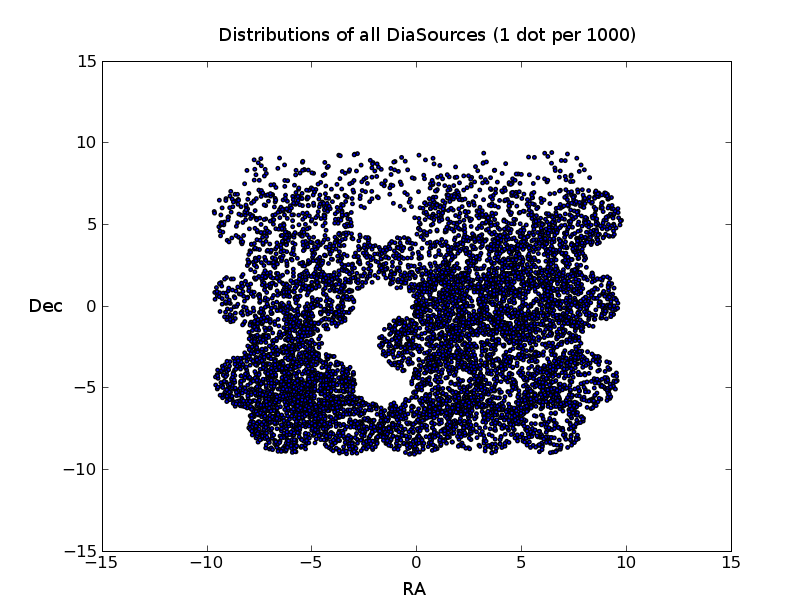
\includegraphics[scale=.7]{illustrations/allDias_1_1000th_density.png}
\caption{A reduced-density plot of simulated asteroid detections (DiaSources) used in our simulated catalog.  Detections from several fields were missing, but we expect that our results should be reasonably representative nonetheless.}
\label{diasPlot}
\end{figure}

A plot of some of the detections used in the simulation is presented
in figure \ref{diasPlot}.  As is visible in the plot, four of the
twenty-two fields had missing data due to a software error.  We expect
that the presence of this flaw in the data should not significantly
affect the conclusions reached from our experiments.



\subsubsubsection{Results}



\begin{figure}[ht!]
\centering \subfloat[Summary of results]{
\begin{tabular}{|r|r|}
%%%%%%%%%%%%%%%%%%%%%%%%%%%%%%%%%%%%%%%%%%%%%%%%%%%%%%%%%%%%%
\hline 
Tracklet generation runtime:  & 2,355 sec  (.6 hours) \\
Track generation runtime:     & 39,713 sec (11 hours) \\
Total linking runtime:        & 42,068 sec (11.7 hours) \\
Peak memory usage:            & 2.2 GB \\
 & \\
Number of tracklets:          & 4,502,224  \\
Tracklet \% true:             & 43.4\% \\
Number of tracks:             & 3,318,539 \\
Track \% true:                & 26.6\% \\
 & \\
Estimated OD cost (assuming 1000 OD/sec):  & 3,318 sec (.9 hours) \\
Estimated total resource usage:      & 45,386 sec (12.6 hours)\\
 & \\
Number of findable objects:   & 186,344 \\
Number of objects found:      & 176,080 \\
\% Found / findable:          & 94.5\% \\
\hline
%%%%%%%%%%%%%%%%%%%%%%%%%%%%%%%%%%%%%%%%%%%%%%%%%%%%%%%%%%%%%
\end{tabular}
}

\subfloat[Found objects by type]{
\begin{tabular}{|r|r|r|r|}
\hline
Object class            & Number found & Number findable & Percent found/findable \\
\hline
Main-belt objects       & 172,539   &  182,285     & 94.7\%  \\
Near-earth objects      & 276       &  504         & 54.8\%        \\
Comets                  & 1,374     &  1,534       & 89.6\%      \\
Trojans                 & 1,593     &  1,696       & 93.9\%      \\
Trans-Neptunian objects & 254       &   281        & 90.4\%      \\
Scattered disk objects  & 44        &    44        & 100\%       \\
\hline
\end{tabular}
}

\caption{In-depth results from our simulated survey of full-density asteroid sources from a subset of the visible sky.}
\label{bigSimResults}
\end{figure}

Our simulated survey was run using a single 2.2 GHz Opteron core.
Results from our simulated survey are presented in figure
\ref{bigSimResults}.  Our success rate for discovery of findable
objects was quite high (just below 95\%) and the number of tracks
generated was reasonably small, meaning that running OD on the output
should not be computationally expensive.  This is a significant
difference from the experiences reported by the PanSTARRS MOPS, in
which OD is considered to be the most expensive phase of processing.
This is because the PanSTARRS MOPS uses a more permissive RMS filter
where our simulation used a less permissive chi-squared
probability-based filter, greatly reducing the number of false tracks.

We also present the types of objects found by class; though our
filters were tuned for main-belt objects, we had a high rate of
success in finding several other types of objects.  Near-earth objects
were underrepresented due to their high velocities; see
\ref{neosTrailing} for future plans to address this.



\subsubsection{Scaling On Solar System Model Density}

To test the scaling of the system as density increases, we generated
``reduced-density'' catalogs.  We randomly chose a subset of the
objects observed in the original catalog and removed all detections of
those objects, then ran DayMOPS on the resulting catalog.  We found
that our software continued to find nearly all the remaining findable
objects regardless of density, though the linking runtimes increased
significantly as density increased. See figure \ref{ssmDensity} for
results.


\begin{figure}
\centering
\subfloat{
\footnotesize
\begin{tabular}{|c|r|r|r|r|r|r|}
  \hline 
  SSM Density & \#DiaSources & \#Tracklets & \#Tracks & Linking Runtime (sec) & Track \% True & Found/Findable   \\
  \hline
  .1        & 827021  &   211,635    & 122,160   & 669         & 75.97\%  & 95.31\% \\
  .025      & 2070722 &   649,907    & 401,895   & 3,664        & 57.94\%  & 94.71\% \\
  .05       & 4140278 & 1,618,205    & 1,116,346 & 17,304       & 40.70\%  & 94.91\% \\
  .75       & 6197009 & 2,897,291    & 2,085,296 & 46,077       & 32.14\%  & 94.74\% \\
  1.0       & 8274898 & 4,502,224    & 3,318,420 & 98,848       & 26.61\%  & 94.56\% \\
  \hline
\end{tabular}
}







\subfloat{
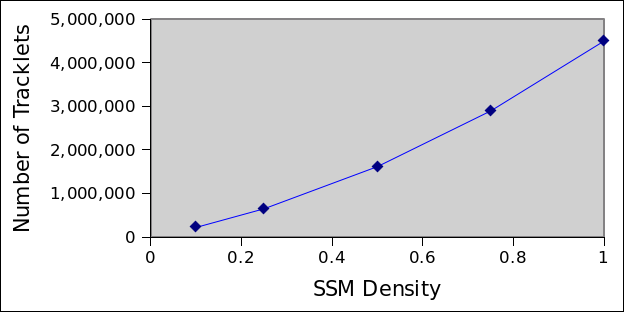
\includegraphics[scale=.4]{illustrations/density_v_nTracklets.png}
}
\subfloat{
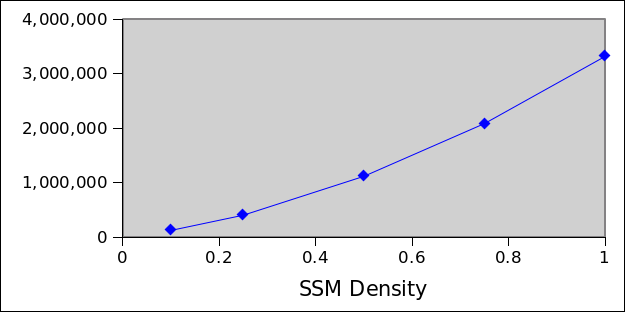
\includegraphics[scale=.4]{illustrations/density_v_nTracks.png}
}


\subfloat{
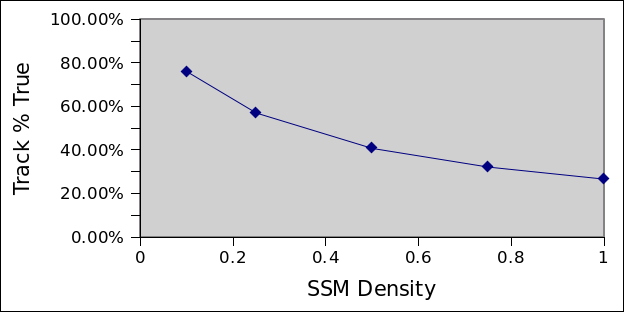
\includegraphics[scale=.4]{illustrations/density_v_trackTrue.png}
}
\subfloat{
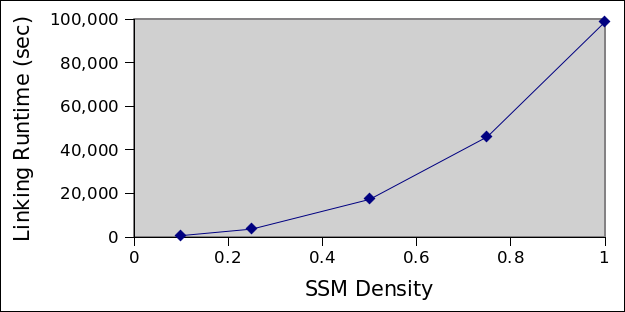
\includegraphics[scale=.4]{illustrations/density_v_runtime.png}
}


\caption{ Results from running DayMOPS linking methods on reduced-density source catalogs. }

\label{ssmDensity}

\end{figure}














\subsubsection{Scaling On Non-Solar System Detection Density}

Even after removal of background stars, actual observational data will
include a variety of non-asteroid sources, including transient
phenomena and image processing artifacts.  In order to estimate the
tolerance of DayMOPS linking methods to these sources, we carried out
a series of simulated surveys which included varying numbers of
randomly-distributed ``noise'' sources throughout each simulated
image.  To reduce the runtime of the experiment, the asteroid
detection catalog was taken from the 50\%-density SSM catalog from the
prior experiment.  The addition of noise had little impact on the
ability of the software to find nearly all the findable objects, but
did result in increased runtime for the linking phase.  See figure
\ref{noiseDensity} for results.





\begin{figure}

\subfloat{
\footnotesize
\begin{tabular}{|r|r|r|r|r|r|r|}
  \hline 
Noise Points / Image &   \% Noise & \#Tracklets & \#Tracks  & Linking Runtime (sec) & Track \% True & Found/Findable \\
0      &     0.0\%    &  1,618,205  & 1,116,346 & 8,413           &  40.70\%      &  94.91\%       \\
500    &     20.63\%  & 1,947,235   & 1,127,355 & 9,996           & 40.28\%       &  94.90\%       \\
2,500  &     56.51\%  & 4,107,233   & 1,202,270 & 19,321          & 50.36\%       &  94.87\%       \\
5,000  &     72.21\%  & 8,693,128   & 1,361,796 & 51,008          & 33.14\%       &  94.80\%       \\
10,000 &     83.87\%  & 23,989,975  & 1,951,794 & 256,565         & 22.89\%       &  94.62\%       \\
   \hline
\end{tabular}
}

\subfloat{
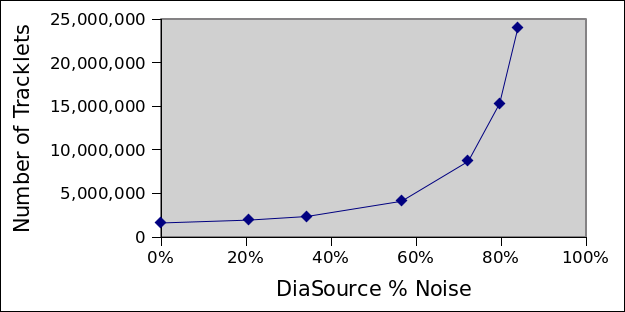
\includegraphics[scale=.4]{illustrations/noise_v_nTracklets.png}
}
\subfloat{
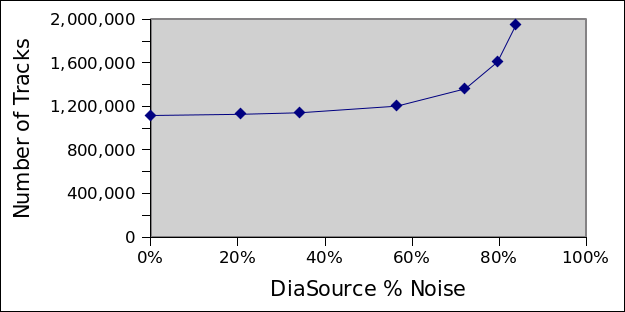
\includegraphics[scale=.4]{illustrations/noise_v_nTracks.png}
}

\subfloat{
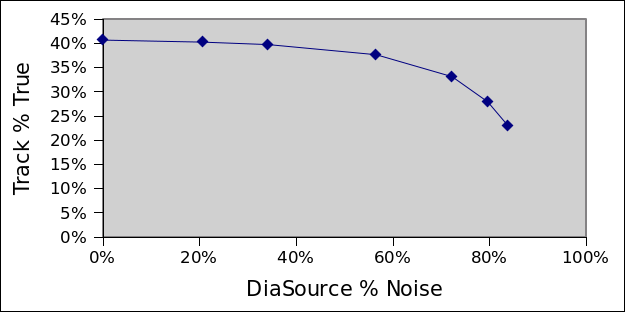
\includegraphics[scale=.4]{illustrations/noise_v_trackTrue.png}
}
\subfloat{
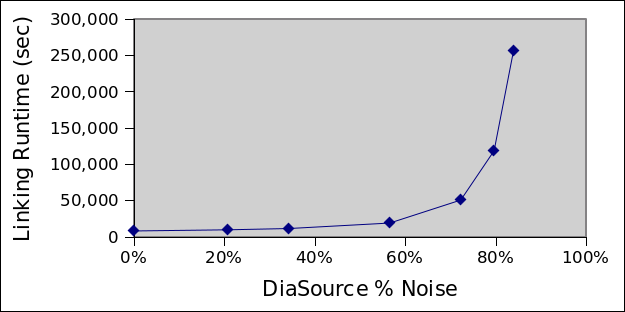
\includegraphics[scale=.4]{illustrations/noise_v_runtime.png}
}

\caption{Results from a simulated survey using a 50\%-density SSM and
  varying numbers of randomly-distributed ``noise'' (non-asteroid)
  sources per image.}
\label{noiseDensity}
\end{figure}






\subsection{NightMOPS Resource Usage}

The costs of running NightMOPS are expected to be negligable compared
with the costs of running DayMOPS.  NightMOPS (fed from a database of
real known objects) has been run in past data challenges and has not
imposed a significant cost. 











\section{Implications for Telescope Cadence}
\label{cadenceRequirements}

\subsection{Cadence Requirements Imposed by Sky-Plane Linking Methods}

The multi-tiered approach we describe imposes certain requirements on
telescope cadence.  For example, we cannot generate a tracklet for an
object unless it is observed twice on a given night; a track cannot be
generated for an object unless it generates multiple tracklets within
a reasonable period of time.

Further practical considerations impose further requirements on
cadence. Even if an object is observed twice within a night, it may
not be practical to generate a tracklet for that object if the time
interval between observations is too large.  This is because within a
large time period, objects can move a significant distance, and the
search space for tracklet generation can become very large, leading to
large numbers of mislinkages.  A casual study in \citet{kubica_thesis}
and experiences related to us from work on the PanSTARRS MOPS both
state an upper time limit of 90 minutes is necessary to prevent
excessively high numbers of mislinkages. A 15-minute lower limit was
also suggested as a minimum for most objects to generate useful
apparent motion relative to astrometric errors. Similarly, the
quadratic approximation of asteroid sky-plane motion breaks down after
periods longer than roughly one month \citep{kubica_thesis}.  As a
result, it is not possible to form tracks from tracklets separated by
greater than one month of observation time.

As mentioned in \ref{orbitFitting}, it is generally held that most
orbit determination methods can generate a reliable orbit given six
detections of an object occuring on at least three distinct nights.
As a general rule, the telescope cadence will attempt to revisit
fields of sky twice on a single night within the aforementioned 15-90
minute interval; it will then attempt to revisit these fields again on
two more nights within a span of 30 days or less.  In this way, and
objects in that field will be observed a total of at least six times
on at least three different nights, generating three or more tracklets
sufficient for linking into a track.


The current implementation of simulated telescope operations
take into account these requirements when generating simulated sets of
telescope pointings. 










\section{Development Plan}

Though the core algorithms of MOPS have been implemented in
LSST-appropriate style, further research and development are needed.



\subsection{Long Duration Survey Performance}

Current simulations cover fairly short time periods, and therefore
emphasize the problem of initial object discovery.  In the course of
the full survey, we expect that many detected sources will be
attributed to already-discovered objects.  Because initial object
discovery phases are relatively expensive and ephemeris calculation is
relatively fast, we expect that the resource usage of the system will
decline over time, as more objects are discovered and the size of
input catalogs is reduced.  This expectation needs to be verified and
quantified.

Attribution, precovery and Moving Object management and refinement of the
Moving Object table are not yet implemented in LSST-compliant software.
Developing this software should be a significant development task.
However, we hope that by using the algorithms from the PanSTARRS MOPS
we can avoid any significant research tasks.

To test this software, we will need to generate simulated input
catalogs which span longer time periods.  Accomplishing this will
require either significant compute-resources or improved tools for
generating input catalogs.



\subsection{Filtering on Trailing for Near-Earth-Object Searching}

\label{neosTrailing}

Near-Earth Objects tend to have the highest sky-plane velocity.  This
presents a significant challenge; as we increase the maximum velocity
limit of our tracklet generation, the potential for mislinkage
increases significantly, leading to higher numbers of tracklets and
increased costs.  

Fortunately, fast-moving NEOs will generate visible trails in our
images.  By requiring all tracklets to show trails consistent with
their apparent sky-plane velocity, we expect that it will be possible
to filter most false tracklet linkages, thus rendering the problem of
NEO searching manageable.

The ability to filter on trailing is dependent almost entirely on our
ability to correctly identify trails in images.  Currently, the
ability of image processing to detect trails is not well quantified.  To
remedy this, we will need to generate simulated images which include
asteroid trails and send them to image processing; further refinement
of image processing algorithms may be neccesary.



\subsection{Distribution/Parallelization of Software}

Current software implementations and simulations presented in this
document use only a single processor.  Performance has been
sufficiently fast for this to be reasonable; however, as we increase
the size of the simulated sky, extend the linking window, and increase
non-asteroid source density, it will likely become necessary to
parallelize some core algorithms.

The PanSTARRS MOPS can inform our decisions on parallelization and
distribution.  Some phases of processing are trivially parallel, such
as Initial Orbit Determination, in which the same operations are
performed to a large variety of tracks; this should be very easy to
accomplish in using LSST Pipeline Middleware.  

Other tasks will be more difficult; in distributing sky-plane linking,
PanSTARRS MOPS divides up the data by field of view and distributes
the workload along this axis.  This has the advantage of distributing
the workload in a straightforward way, but potentially generating
poorly load-balanced workloads.  We plan to investigate this method,
but leave open the possibility of attempting other approaches as well.


\bibliographystyle{apj}
\bibliography{baseline}

\end{document}
